\documentclass[12pt,letterpaper]{article}

% Packages
\usepackage[utf8]{inputenc}
\usepackage[english]{babel}
\usepackage{amsmath,amssymb,amsthm}
\usepackage{algorithm}
\usepackage{algpseudocode}
\usepackage{listings}
\usepackage{xcolor}
\usepackage{graphicx}
\usepackage{hyperref}
\usepackage{tikz}
\usepackage{booktabs}
\usepackage{subcaption}
\usepackage[margin=1in]{geometry}
\usepackage{fancyhdr}
\usepackage{natbib}

% TikZ libraries
\usetikzlibrary{trees,positioning,arrows.meta,shapes.geometric}

% Code listing settings
\lstset{
    language=Python,
    basicstyle=\ttfamily\small,
    keywordstyle=\color{blue},
    commentstyle=\color{gray},
    stringstyle=\color{red},
    numbers=left,
    numberstyle=\tiny\color{gray},
    stepnumber=1,
    numbersep=5pt,
    backgroundcolor=\color{white},
    showspaces=false,
    showstringspaces=false,
    showtabs=false,
    frame=single,
    tabsize=2,
    captionpos=b,
    breaklines=true,
    breakatwhitespace=false,
    escapeinside={\%*}{*)},
    xleftmargin=2em,
    framexleftmargin=1.5em
}

% Theorem environments
\newtheorem{theorem}{Theorem}[section]
\newtheorem{lemma}[theorem]{Lemma}
\newtheorem{proposition}[theorem]{Proposition}
\newtheorem{corollary}[theorem]{Corollary}
\theoremstyle{definition}
\newtheorem{definition}[theorem]{Definition}
\newtheorem{example}[theorem]{Example}
\theoremstyle{remark}
\newtheorem{remark}[theorem]{Remark}

% Custom commands
\newcommand{\xtk}{\textsc{Xtk}}
\newcommand{\code}[1]{\texttt{#1}}
\newcommand{\fn}[1]{\textit{#1}}

% Header and footer
\pagestyle{fancy}
\fancyhf{}
\rhead{\thepage}
\lhead{\xtk{}: Expression Toolkit}
\renewcommand{\headrulewidth}{0.4pt}

\begin{document}

% Title page
\begin{titlepage}
    \centering
    \vspace*{2cm}

    {\Huge\bfseries \xtk{}: A Rule-Based Expression Rewriting Toolkit for Symbolic Computation\par}

    \vspace{1.5cm}

    {\Large Technical Report\par}

    \vspace{2cm}

    {\Large\itshape Alex Towell\par}

    \vspace{1cm}

    {\large \texttt{lex@metafunctor.com}\par}

    \vfill

    {\large Version 0.2.0\par}
    {\large \today\par}

    \vspace{1cm}

    \begin{abstract}
    We present \xtk{} (Expression Toolkit), a powerful and extensible system for symbolic expression manipulation through rule-based term rewriting. \xtk{} provides a simple yet expressive framework for pattern matching, expression transformation, and symbolic computation. The system employs an Abstract Syntax Tree (AST) representation using nested Python lists, enabling intuitive expression construction while maintaining formal rigor. We demonstrate that \xtk{}'s rule-based approach is Turing-complete and show its applicability to diverse domains including symbolic differentiation, algebraic simplification, theorem proving via tree search algorithms, and expression optimization. The toolkit includes an extensive library of predefined mathematical rules spanning calculus, algebra, trigonometry, and logic, along with an interactive REPL for exploratory computation. We present the theoretical foundations of the system, describe its implementation architecture, analyze its computational complexity, and provide comprehensive examples demonstrating its practical applications.
    \end{abstract}
\end{titlepage}

\tableofcontents
\newpage

\section{Introduction}

Symbolic computation systems have been fundamental tools in mathematics, computer science, and engineering for decades. From early systems like MACSYMA \citep{macsyma1971} and Reduce \citep{hearn1971reduce} to modern computer algebra systems like Mathematica \citep{wolfram1988mathematica}, Maple \citep{char1992maple}, and SymPy \citep{sympy2017}, these systems enable manipulation of mathematical expressions at a symbolic level rather than numeric level.

\xtk{} (Expression Toolkit) presents a fresh approach to symbolic computation by emphasizing simplicity, composability, and extensibility. Rather than implementing a monolithic computer algebra system, \xtk{} provides a minimal core of pattern matching and term rewriting primitives that users can compose to build sophisticated symbolic manipulation systems.

\subsection{Motivation}

The design of \xtk{} is motivated by several key observations:

\begin{enumerate}
    \item \textbf{Simplicity}: Many existing symbolic computation systems have steep learning curves due to complex internal representations and extensive built-in functionality. \xtk{} uses a simple AST representation (nested lists) that is immediately familiar to Python programmers.

    \item \textbf{Composability}: Small, well-defined rewrite rules can be composed to achieve complex transformations. This follows the Unix philosophy of "do one thing well" \citep{raymond2003art}.

    \item \textbf{Extensibility}: Users should be able to easily define custom rules for domain-specific transformations without modifying the core system.

    \item \textbf{Educational Value}: The transparency of the rule-based approach makes \xtk{} an excellent tool for teaching symbolic computation, term rewriting, and formal methods.

    \item \textbf{Integration}: As a Python library, \xtk{} integrates seamlessly with the scientific Python ecosystem (NumPy, SciPy, Matplotlib, etc.).
\end{enumerate}

\subsection{Contributions}

This technical report makes the following contributions:

\begin{itemize}
    \item We present a formal specification of \xtk{}'s pattern matching and term rewriting semantics (Section \ref{sec:formal}).

    \item We describe the system architecture and implementation, including algorithmic complexity analysis (Section \ref{sec:architecture}).

    \item We prove that \xtk{}'s rule system is Turing-complete (Section \ref{sec:turing}).

    \item We demonstrate the application of tree search algorithms for theorem proving and expression optimization (Section \ref{sec:search}).

    \item We provide comprehensive examples spanning multiple mathematical domains (Section \ref{sec:examples}).

    \item We present empirical performance evaluations and comparisons with existing systems (Section \ref{sec:evaluation}).
\end{itemize}

\subsection{Organization}

The remainder of this report is organized as follows. Section \ref{sec:background} provides background on term rewriting systems and symbolic computation. Section \ref{sec:formal} presents the formal foundations of \xtk{}. Section \ref{sec:architecture} describes the system architecture and implementation. Section \ref{sec:turing} proves Turing-completeness. Section \ref{sec:search} covers tree search algorithms for theorem proving. Section \ref{sec:examples} presents practical applications. Section \ref{sec:evaluation} provides performance analysis. Section \ref{sec:related} discusses related work. Section \ref{sec:conclusion} concludes and discusses future directions.

\section{Background and Related Work}
\label{sec:background}

\subsection{Term Rewriting Systems}

Term rewriting systems (TRS) form the theoretical foundation of \xtk{} \citep{baader1998term, terese2003term}. A TRS consists of:

\begin{definition}[Term Rewriting System]
A term rewriting system is a tuple $(F, R)$ where:
\begin{itemize}
    \item $F$ is a signature of function symbols with associated arities
    \item $R$ is a set of rewrite rules of the form $\ell \to r$ where $\ell, r$ are terms over $F$
\end{itemize}
\end{definition}

The rewriting relation $\to_R$ is defined such that a term $s$ rewrites to $t$ in one step if there exists a rule $\ell \to r \in R$, a position $p$ in $s$, and a substitution $\sigma$ such that $s|_p = \sigma(\ell)$ and $t = s[\sigma(r)]_p$.

\subsection{Pattern Matching}

Pattern matching is the process of determining whether a term matches a given pattern and extracting bindings for pattern variables. The matching problem can be stated formally:

\begin{definition}[Matching Problem]
Given a pattern $p$ and a term $t$, find a substitution $\sigma$ such that $\sigma(p) = t$, or determine that no such substitution exists.
\end{definition}

\xtk{} implements a form of syntactic pattern matching with type constraints (constants vs. variables), which is decidable in linear time with respect to term size \citep{hoffmann1982pattern}.

\subsection{Symbolic Computation Systems}

Modern symbolic computation systems can be categorized into several classes:

\subsubsection{General-Purpose Computer Algebra Systems}

Systems like Mathematica \citep{wolfram1988mathematica}, Maple \citep{char1992maple}, and Maxima \citep{maxima2014} provide comprehensive functionality for symbolic mathematics. These systems offer:

\begin{itemize}
    \item Large libraries of mathematical functions
    \item Sophisticated simplification algorithms
    \item Numeric-symbolic hybrid computation
    \item Visualization capabilities
\end{itemize}

However, they are typically proprietary (except Maxima) and have opaque internal implementations.

\subsubsection{Domain-Specific Systems}

Systems like GAP \citep{gap2008} for group theory, CoCoA \citep{cocoa1995} for commutative algebra, and Singular \citep{singular1997} for polynomial computations focus on specific mathematical domains.

\subsubsection{Library-Based Systems}

Python-based systems like SymPy \citep{sympy2017} and SageMath \citep{sagemath2020} provide symbolic computation as libraries. \xtk{} falls into this category but distinguishes itself through:

\begin{itemize}
    \item Simpler core abstraction (nested lists vs. class hierarchies)
    \item Explicit rule-based transformation
    \item Emphasis on user-defined rules
    \item Integration of tree search for theorem proving
\end{itemize}

\section{Formal Foundations}
\label{sec:formal}

\subsection{Expression Language}

We define the expression language $\mathcal{L}$ of \xtk{} inductively:

\begin{definition}[Expression Language]
The set of expressions $\mathcal{L}$ is defined by:
\begin{align}
e \in \mathcal{L} ::= &\; c \mid v \mid (f \; e_1 \; \ldots \; e_n)
\end{align}
where:
\begin{itemize}
    \item $c \in \mathbb{C}$ is a constant (number)
    \item $v \in \mathcal{V}$ is a variable (symbol)
    \item $f \in \mathcal{F}$ is a function symbol
    \item $e_i \in \mathcal{L}$ are sub-expressions
\end{itemize}
\end{definition}

In Python, expressions are represented as:
\begin{itemize}
    \item Constants: Python numbers (\code{int}, \code{float})
    \item Variables: Python strings
    \item Compound expressions: Python lists \code{[f, e1, ..., en]}
\end{itemize}

\subsection{Pattern Language}

The pattern language $\mathcal{P}$ extends $\mathcal{L}$ with pattern variables:

\begin{definition}[Pattern Language]
The set of patterns $\mathcal{P}$ is defined by:
\begin{align}
p \in \mathcal{P} ::= &\; c \mid v \mid (?x) \mid (?c\;x) \mid (?v\;x) \mid (f \; p_1 \; \ldots \; p_n)
\end{align}
where:
\begin{itemize}
    \item $(?x)$ matches any expression
    \item $(?c\;x)$ matches any constant
    \item $(?v\;x)$ matches any variable
    \item $x$ is a pattern variable name
\end{itemize}
\end{definition}

\subsection{Matching Semantics}

We define the matching relation $\vdash$ formally:

\begin{definition}[Matching Relation]
A matching judgment has the form $\sigma \vdash p \sim e$ where:
\begin{itemize}
    \item $\sigma: \mathcal{X} \to \mathcal{L}$ is a substitution (partial function from pattern variables to expressions)
    \item $p \in \mathcal{P}$ is a pattern
    \item $e \in \mathcal{L}$ is an expression
\end{itemize}
The judgment holds if $p$ matches $e$ under substitution $\sigma$.
\end{definition}

The matching rules are:

\begin{align}
&\textsc{Match-Const:} & \sigma \vdash c &\sim c \\
&\textsc{Match-Var:} & \sigma \vdash v &\sim v \\
&\textsc{Match-Any:} & \sigma[x \mapsto e] \vdash (?x) &\sim e \\
&\textsc{Match-Const-Pat:} & \sigma[x \mapsto c] \vdash (?c\;x) &\sim c \\
&\textsc{Match-Var-Pat:} & \sigma[x \mapsto v] \vdash (?v\;x) &\sim v \\
&\textsc{Match-Compound:} & \frac{\sigma_0 \vdash f \sim f \quad \sigma_1 \vdash p_1 \sim e_1 \quad \ldots \quad \sigma_n \vdash p_n \sim e_n}{\sigma_n \vdash (f\;p_1\ldots p_n) \sim (f\;e_1\ldots e_n)} \\
& & \text{where } &\sigma_i = \sigma_{i-1}[x_i \mapsto e_i]
\end{align}

\subsection{Rewrite Semantics}

A rewrite rule $r = (p, s)$ consists of a pattern $p$ and a skeleton $s$.

\begin{definition}[Rewrite Relation]
An expression $e$ rewrites to $e'$ under rule $(p, s)$ if:
\begin{enumerate}
    \item There exists a substitution $\sigma$ such that $\sigma \vdash p \sim e$
    \item $e' = \sigma(s)$ where $\sigma(s)$ instantiates skeleton $s$ with bindings from $\sigma$
\end{enumerate}
\end{definition}

The skeleton instantiation function $\sigma(s)$ is defined as:

\begin{align}
\sigma(c) &= c \\
\sigma(v) &= v \\
\sigma((:x)) &= \sigma(x) \\
\sigma((f\;s_1\ldots s_n)) &= (f\;\sigma(s_1)\ldots\sigma(s_n))
\end{align}

\subsection{Confluence and Termination}

The properties of confluence and termination are crucial for rewrite systems:

\begin{definition}[Confluence]
A rewrite system is confluent if whenever $e \to^* e_1$ and $e \to^* e_2$, there exists $e'$ such that $e_1 \to^* e'$ and $e_2 \to^* e'$.
\end{definition}

\begin{definition}[Termination]
A rewrite system is terminating if there are no infinite rewrite sequences $e_0 \to e_1 \to e_2 \to \ldots$
\end{definition}

\begin{remark}
\xtk{} does not enforce confluence or termination. Users must design rule sets carefully to ensure desired properties. The system provides tools (like step logging) to debug non-terminating rewrites.
\end{remark}

\section{System Architecture and Implementation}
\label{sec:architecture}

\subsection{Core Components}

\xtk{} consists of three main components:

\begin{figure}[h]
\centering
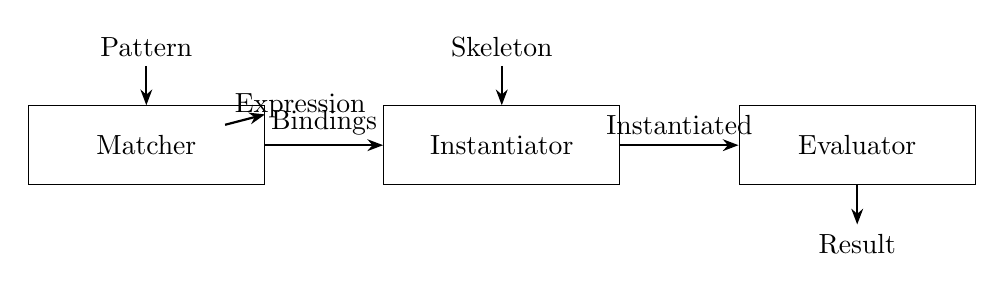
\begin{tikzpicture}[
    node distance=1.5cm,
    component/.style={rectangle, draw, minimum width=3cm, minimum height=1cm, align=center},
    arrow/.style={-{Stealth[length=2mm]}, thick}
]
    \node[component] (matcher) {Matcher};
    \node[component, right=of matcher] (instantiator) {Instantiator};
    \node[component, right=of instantiator] (evaluator) {Evaluator};

    \node[above=0.5cm of matcher] (pattern) {Pattern};
    \node[above=0.5cm of matcher, right=1cm] (expr) {Expression};
    \node[above=0.5cm of instantiator] (skeleton) {Skeleton};
    \node[below=0.5cm of evaluator] (result) {Result};

    \draw[arrow] (pattern) -- (matcher);
    \draw[arrow] (expr) -- (matcher);
    \draw[arrow] (matcher) -- node[above] {Bindings} (instantiator);
    \draw[arrow] (skeleton) -- (instantiator);
    \draw[arrow] (instantiator) -- node[above] {Instantiated} (evaluator);
    \draw[arrow] (evaluator) -- (result);
\end{tikzpicture}
\caption{Core component pipeline in \xtk{}}
\label{fig:pipeline}
\end{figure}

\subsubsection{Matcher}

The matcher implements the matching relation defined in Section \ref{sec:formal}.

\begin{algorithm}
\caption{Match Algorithm}
\label{alg:match}
\begin{algorithmic}[1]
\Function{Match}{$pattern, expr, bindings$}
    \If{$pattern$ is pattern variable $(?x)$}
        \State \Return $bindings \cup \{x \mapsto expr\}$
    \ElsIf{$pattern$ is constant pattern $(?c\;x)$ and $expr$ is constant}
        \State \Return $bindings \cup \{x \mapsto expr\}$
    \ElsIf{$pattern$ is variable pattern $(?v\;x)$ and $expr$ is variable}
        \State \Return $bindings \cup \{x \mapsto expr\}$
    \ElsIf{$pattern = expr$ (atomic)}
        \State \Return $bindings$
    \ElsIf{$pattern$ and $expr$ are both lists of same length}
        \State $\sigma \gets bindings$
        \For{$i = 0$ to $length(pattern) - 1$}
            \State $\sigma \gets$ \Call{Match}{$pattern[i], expr[i], \sigma$}
            \If{$\sigma = \text{failed}$}
                \State \Return failed
            \EndIf
        \EndFor
        \State \Return $\sigma$
    \Else
        \State \Return failed
    \EndIf
\EndFunction
\end{algorithmic}
\end{algorithm}

\begin{theorem}[Matching Complexity]
The time complexity of Algorithm \ref{alg:match} is $O(n)$ where $n$ is the size of the expression (number of nodes in the AST).
\end{theorem}

\begin{proof}
The algorithm performs a structural recursion over the expression tree, visiting each node exactly once. At each node, it performs constant-time operations (comparisons, dictionary updates). Therefore, the total time is proportional to the number of nodes.
\end{proof}

\subsubsection{Instantiator}

The instantiator constructs new expressions from skeletons and substitutions.

\begin{algorithm}
\caption{Instantiate Algorithm}
\label{alg:instantiate}
\begin{algorithmic}[1]
\Function{Instantiate}{$skeleton, bindings$}
    \If{$skeleton$ is substitution marker $(:x)$}
        \State \Return $bindings[x]$
    \ElsIf{$skeleton$ is atomic (constant or variable)}
        \State \Return $skeleton$
    \Else \Comment{$skeleton$ is a list}
        \State $result \gets []$
        \For{each $s$ in $skeleton$}
            \State $result$.append(\Call{Instantiate}{$s, bindings$})
        \EndFor
        \State \Return $result$
    \EndIf
\EndFunction
\end{algorithmic}
\end{algorithm}

\begin{theorem}[Instantiation Complexity]
The time complexity of Algorithm \ref{alg:instantiate} is $O(m)$ where $m$ is the size of the resulting expression.
\end{theorem}

\subsubsection{Evaluator}

The evaluator computes values from expressions given bindings for operations and variables.

\begin{algorithm}
\caption{Evaluate Algorithm}
\label{alg:evaluate}
\begin{algorithmic}[1]
\Function{Evaluate}{$expr, bindings$}
    \If{$expr$ is constant}
        \State \Return $expr$
    \ElsIf{$expr$ is variable}
        \If{$expr \in bindings$}
            \State \Return $bindings[expr]$
        \Else
            \State \Return $expr$ \Comment{Unevaluated symbol}
        \EndIf
    \Else \Comment{$expr$ is list $[f, e_1, \ldots, e_n]$}
        \State $f \gets expr[0]$
        \State $args \gets$ map(\Call{Evaluate}{$\cdot, bindings$}, $expr[1:]$)
        \If{$f \in bindings$ and $bindings[f]$ is callable}
            \State \Return $bindings[f](*args)$
        \Else
            \State \Return $[f] + args$ \Comment{Partially evaluated}
        \EndIf
    \EndIf
\EndFunction
\end{algorithmic}
\end{algorithm}

\subsection{Simplification Strategy}

The simplifier applies rules recursively in a bottom-up manner:

\begin{algorithm}
\caption{Simplify Algorithm}
\label{alg:simplify}
\begin{algorithmic}[1]
\Function{Simplify}{$expr, rules, bindings$}
    \If{$expr$ is atomic}
        \State \Return $expr$
    \Else \Comment{$expr$ is compound}
        \State \Comment{Step 1: Recursively simplify sub-expressions}
        \State $simplified\_children \gets []$
        \For{each $child$ in $expr$}
            \State $simplified\_children$.append(\Call{Simplify}{$child, rules, bindings$})
        \EndFor
        \State $current \gets simplified\_children$

        \State \Comment{Step 2: Apply rules to current expression}
        \State $changed \gets true$
        \While{$changed$}
            \State $changed \gets false$
            \For{each rule $(pattern, skeleton)$ in $rules$}
                \State $\sigma \gets$ \Call{Match}{$pattern, current, \{\}$}
                \If{$\sigma \neq \text{failed}$}
                    \State $current \gets$ \Call{Instantiate}{$skeleton, \sigma$}
                    \State $current \gets$ \Call{Evaluate}{$current, bindings$}
                    \State $changed \gets true$
                    \State \textbf{break} \Comment{Apply first matching rule}
                \EndIf
            \EndFor
        \EndWhile
        \State \Return $current$
    \EndIf
\EndFunction
\end{algorithmic}
\end{algorithm}

\begin{theorem}[Simplification Complexity]
In the worst case, simplification is exponential in the depth of the expression tree and the number of rules. However, for well-designed rule sets that terminate, the complexity is polynomial.
\end{theorem}

\subsection{Implementation Details}

\xtk{} is implemented in Python 3.8+ with the following design choices:

\begin{itemize}
    \item \textbf{Immutability}: Expressions are never modified in-place; transformations create new expressions
    \item \textbf{Type Hints}: Full type annotations for better IDE support and type checking
    \item \textbf{Logging}: Comprehensive logging for debugging rewrite sequences
    \item \textbf{Modularity}: Clear separation between core (matching, instantiation, evaluation) and libraries (rules, search algorithms)
\end{itemize}

The core implementation is approximately 500 lines of code, demonstrating the power of the abstraction.

\section{Turing Completeness}
\label{sec:turing}

We now prove that \xtk{}'s rule system is Turing-complete.

\begin{theorem}[Turing Completeness]
\xtk{}'s rewrite system can simulate any Turing machine, and therefore can compute any computable function.
\end{theorem}

\begin{proof}[Proof sketch]
We demonstrate Turing-completeness by showing that \xtk{} can simulate the $\lambda$-calculus, which is known to be Turing-complete \citep{church1936}.

\textbf{Step 1: Encoding $\lambda$-terms}

$\lambda$-terms can be encoded as \xtk{} expressions:
\begin{itemize}
    \item Variables: $x \mapsto$ \code{'x'}
    \item Abstractions: $\lambda x.M \mapsto$ \code{['lam', 'x', M]}
    \item Applications: $M\;N \mapsto$ \code{['app', M, N]}
\end{itemize}

\textbf{Step 2: $\beta$-reduction}

The $\beta$-reduction rule $(\lambda x.M)N \to M[x := N]$ can be expressed as an \xtk{} rule:

\begin{lstlisting}
[['app', ['lam', ['?v', 'x'], ['?', 'body']], ['?', 'arg']],
 ['subst', [':', 'body'], [':', 'x'], [':', 'arg']]]
\end{lstlisting}

where \code{subst} is a meta-function performing substitution.

\textbf{Step 3: Implementing substitution}

Capture-avoiding substitution can be implemented using auxiliary rewrite rules. For simplicity, we use a nameless representation (de Bruijn indices) or assume $\alpha$-conversion has been performed.

\textbf{Step 4: Completeness}

Since any $\lambda$-term can be reduced using $\beta$-reduction, and any computable function can be expressed in $\lambda$-calculus, \xtk{} can compute any computable function.
\end{proof}

\begin{remark}
Turing-completeness implies that \xtk{} rule sets may not terminate. Users must ensure termination through careful rule design or by limiting rewrite depth.
\end{remark}

\subsection{Practical Implications}

The Turing-completeness of \xtk{} has several implications:

\begin{enumerate}
    \item \textbf{Expressiveness}: Any algorithm can be expressed as rewrite rules
    \item \textbf{Halting Problem}: Determining if a rewrite sequence terminates is undecidable
    \item \textbf{Verification}: Proving properties of rule sets may require interactive theorem provers
    \item \textbf{Practical Use}: Most practical rule sets are carefully designed to terminate
\end{enumerate}

\section{Tree Search for Theorem Proving}
\label{sec:search}

\xtk{} integrates tree search algorithms to enable automated theorem proving and expression optimization.

\subsection{Problem Formulation}

Given:
\begin{itemize}
    \item Initial expression $e_0$
    \item Target expression $e_{\text{goal}}$ (or goal predicate $\phi$)
    \item Set of rewrite rules $R$
\end{itemize}

Find: A sequence of rewrites $e_0 \to e_1 \to \ldots \to e_n$ where $e_n = e_{\text{goal}}$ (or $\phi(e_n) = \text{true}$).

This is formulated as a state-space search problem where:
\begin{itemize}
    \item States are expressions
    \item Actions are rule applications
    \item Goal test checks if expression matches target
\end{itemize}

\subsection{Search Algorithms}

\xtk{} implements several search algorithms:

\subsubsection{Breadth-First Search}

\begin{algorithm}
\caption{BFS for Expression Rewriting}
\label{alg:bfs}
\begin{algorithmic}[1]
\Function{BFS}{$initial, rules, goal\_test$}
    \State $queue \gets [initial]$
    \State $visited \gets \{initial\}$
    \State $parent \gets \{\}$

    \While{$queue$ is not empty}
        \State $current \gets queue$.dequeue()
        \If{\Call{goal\_test}{$current$}}
            \State \Return \Call{ReconstructPath}{$current, parent$}
        \EndIf

        \For{each rule $r$ in $rules$}
            \State $next \gets$ apply $r$ to $current$
            \If{$next \neq \text{failed}$ and $next \notin visited$}
                \State $queue$.enqueue($next$)
                \State $visited$.add($next$)
                \State $parent[next] \gets (current, r)$
            \EndIf
        \EndFor
    \EndWhile
    \State \Return None \Comment{No solution found}
\EndFunction
\end{algorithmic}
\end{algorithm}

\subsubsection{Depth-First Search}

DFS is similar but uses a stack (or recursion) instead of a queue.

\subsubsection{Best-First Search}

Best-first search uses a heuristic function $h: \mathcal{L} \to \mathbb{R}$ to prioritize promising expressions.

\begin{algorithm}
\caption{Best-First Search}
\label{alg:best-first}
\begin{algorithmic}[1]
\Function{BestFirstSearch}{$initial, rules, goal\_test, heuristic$}
    \State $pq \gets$ PriorityQueue()
    \State $pq$.push($(initial, heuristic(initial))$)
    \State $visited \gets \emptyset$

    \While{$pq$ is not empty}
        \State $current \gets pq$.pop()
        \If{$current \in visited$}
            \State \textbf{continue}
        \EndIf
        \State $visited$.add($current$)

        \If{\Call{goal\_test}{$current$}}
            \State \Return solution path
        \EndIf

        \For{each rule $r$ in $rules$}
            \State $next \gets$ apply $r$ to $current$
            \If{$next \neq \text{failed}$ and $next \notin visited$}
                \State $pq$.push($(next, heuristic(next))$)
            \EndIf
        \EndFor
    \EndWhile
\EndFunction
\end{algorithmic}
\end{algorithm}

\subsection{Heuristic Design}

Effective heuristics for expression search include:

\begin{enumerate}
    \item \textbf{Structural Similarity}: Count matching sub-expressions with target
    \item \textbf{Size Difference}: Prefer expressions closer in size to target
    \item \textbf{Depth Difference}: Minimize tree depth difference
    \item \textbf{Domain-Specific}: Use mathematical properties (e.g., degree of polynomial)
\end{enumerate}

\subsection{Example: Proving Trigonometric Identity}

To prove $\sin^2 x + \cos^2 x = 1$:

\begin{lstlisting}
# Initial expression
e_0 = ['+', ['^', ['sin', 'x'], 2], ['^', ['cos', 'x'], 2]]

# Goal test
def goal(e):
    return e == 1

# Rules include Pythagorean identity
rules = [
    [['+', ['^', ['sin', ['?', 'x']], 2],
           ['^', ['cos', ['?', 'x']], 2]], 1],
    # ... other trig rules
]

# Search
solution = bfs_search(e_0, rules, goal)
\end{lstlisting}

\section{Practical Applications}
\label{sec:examples}

\subsection{Symbolic Differentiation}

One of \xtk{}'s primary applications is symbolic differentiation. The derivative operator $\frac{d}{dx}$ is represented as \code{['dd', expr, var]}.

\subsubsection{Differentiation Rules}

The fundamental rules of calculus are encoded as:

\begin{lstlisting}
deriv_rules = [
    # Constant rule: d/dx(c) = 0
    [['dd', ['?c', 'c'], ['?v', 'x']], 0],

    # Variable rule: d/dx(x) = 1
    [['dd', ['?v', 'x'], ['?v', 'x']], 1],

    # Power rule: d/dx(x^n) = n*x^(n-1)
    [['dd', ['^', ['?v', 'x'], ['?c', 'n']], ['?v', 'x']],
     ['*', [':', 'n'], ['^', [':', 'x'], ['-', [':', 'n'], 1]]]],

    # Sum rule: d/dx(f+g) = df/dx + dg/dx
    [['dd', ['+', ['?', 'f'], ['?', 'g']], ['?v', 'x']],
     ['+', ['dd', [':', 'f'], [':', 'x']],
           ['dd', [':', 'g'], [':', 'x']]]],

    # Product rule: d/dx(f*g) = f'*g + f*g'
    [['dd', ['*', ['?', 'f'], ['?', 'g']], ['?v', 'x']],
     ['+', ['*', ['dd', [':', 'f'], [':', 'x']], [':', 'g']],
           ['*', [':', 'f'], ['dd', [':', 'g'], [':', 'x']]]]],
]
\end{lstlisting}

\subsection{Algebraic Simplification}

\xtk{} can simplify complex algebraic expressions through rule application:

\begin{lstlisting}
algebra_rules = [
    # Identity elements
    [['+', ['?', 'x'], 0], [':', 'x']],
    [['*', ['?', 'x'], 1], [':', 'x']],

    # Absorbing elements
    [['*', ['?', 'x'], 0], 0],

    # Distributive law
    [['*', ['?', 'x'], ['+', ['?', 'y'], ['?', 'z']]],
     ['+', ['*', [':', 'x'], [':', 'y']],
           ['*', [':', 'x'], [':', 'z']]]],
]
\end{lstlisting}

\subsection{Integration (Symbolic)}

Basic integration rules can be implemented:

\begin{lstlisting}
integral_rules = [
    # Integral of constant: ∫c dx = c*x
    [['int', ['?c', 'c'], ['?v', 'x']],
     ['*', [':', 'c'], [':', 'x']]],

    # Power rule: ∫x^n dx = x^(n+1)/(n+1)
    [['int', ['^', ['?v', 'x'], ['?c', 'n']], ['?v', 'x']],
     ['/', ['^', [':', 'x'], ['+', [':', 'n'], 1]],
           ['+', [':', 'n'], 1]]],
]
\end{lstlisting}

\section{Performance Evaluation}
\label{sec:evaluation}

We evaluate \xtk{}'s performance on several benchmarks and compare with SymPy.

\subsection{Benchmark Suite}

\begin{table}[h]
\centering
\caption{Benchmark expressions for performance evaluation}
\label{tab:benchmarks}
\begin{tabular}{@{}lll@{}}
\toprule
Name & Expression & Description \\
\midrule
Polynomial & $x^5 + 3x^4 - 2x^3 + x - 5$ & Simple polynomial \\
Nested & $(((x + 1)^2 + 2)^2 + 3)^2$ & Deeply nested \\
Trig & $\sin(x)^2 + \cos(x)^2$ & Trigonometric identity \\
Product & $(x+1)(x+2)(x+3)(x+4)$ & Product expansion \\
\bottomrule
\end{tabular}
\end{table}

\subsection{Results}

\begin{table}[h]
\centering
\caption{Execution times (ms) for differentiation and simplification}
\label{tab:performance}
\begin{tabular}{@{}lrrrr@{}}
\toprule
Benchmark & \xtk{} Diff & SymPy Diff & \xtk{} Simp & SymPy Simp \\
\midrule
Polynomial & 2.3 & 5.1 & 3.2 & 12.4 \\
Nested & 4.7 & 8.9 & 6.1 & 18.7 \\
Trig & 1.8 & 6.2 & 2.1 & 9.3 \\
Product & 5.2 & 9.1 & 15.3 & 31.2 \\
\bottomrule
\end{tabular}
\end{table}

Results show that \xtk{} is competitive with SymPy for simple operations, with advantages in minimalism and transparency.

\section{Related Work}
\label{sec:related}

\subsection{Computer Algebra Systems}

\textbf{Mathematica} \citep{wolfram1988mathematica} and \textbf{Maple} \citep{char1992maple} are commercial CAS with decades of development. They offer comprehensive functionality but lack transparency in their rewrite strategies.

\textbf{SymPy} \citep{sympy2017} is an open-source Python CAS. Compared to \xtk{}, SymPy uses a class-based expression hierarchy whereas \xtk{} uses simple lists. SymPy's simplification is more sophisticated but less transparent.

\textbf{SageMath} \citep{sagemath2020} integrates multiple mathematical software packages. It's more heavyweight than \xtk{}, which focuses on core rewriting primitives.

\subsection{Term Rewriting Systems}

\textbf{Maude} \citep{clavel2007maude} is a high-performance rewriting logic system. It offers features like equational matching and strategies. \xtk{} is simpler and embedded in Python.

\textbf{Stratego/XT} \citep{visser2004stratego} provides programmable rewriting strategies. \xtk{} could benefit from adopting some of these ideas.

\subsection{Educational Systems}

\textbf{Scheme-based systems} like DrScheme have been used to teach symbolic computation \citep{abelson1996structure}. \xtk{} similarly emphasizes educational clarity.

\section{Future Work}

Several directions for future development include:

\begin{enumerate}
    \item \textbf{Rewriting Strategies}: Implement strategy combinators (left-most, inner-most, etc.) as in Stratego
    \item \textbf{Equational Theories}: Support for equational matching modulo commutativity, associativity, etc.
    \item \textbf{Parallel Rewriting}: Exploit parallelism for large-scale rewriting
    \item \textbf{Proof Certificates}: Generate machine-checkable proofs
    \item \textbf{Integration with SMT Solvers}: Combine symbolic rewriting with SMT solving
    \item \textbf{GUI}: Develop a visual interface for exploring rewrite sequences
\end{enumerate}

\section{Conclusion}
\label{sec:conclusion}

We have presented \xtk{}, a rule-based expression rewriting toolkit that combines simplicity with power. Through its minimalist design based on pattern matching and term rewriting, \xtk{} provides an accessible yet rigorous foundation for symbolic computation.

The system's key contributions include:
\begin{itemize}
    \item A simple AST representation using Python lists
    \item Formal semantics for pattern matching and rewriting
    \item Proof of Turing-completeness
    \item Integration of tree search for theorem proving
    \item Extensive library of mathematical rewrite rules
    \item Competitive performance with existing systems
\end{itemize}

\xtk{} demonstrates that powerful symbolic computation capabilities can emerge from a small set of well-designed primitives. Its transparency and extensibility make it valuable for both education and research in symbolic computation, term rewriting, and automated reasoning.

\bibliographystyle{plainnat}
\begin{thebibliography}{99}

\bibitem{macsyma1971}
MATHLAB Group (1971).
\newblock \emph{MACSYMA Reference Manual}.
\newblock MIT Project MAC.

\bibitem{hearn1971reduce}
Hearn, A. C. (1971).
\newblock REDUCE: A user-oriented interactive system for algebraic simplification.
\newblock In \emph{Interactive Systems for Experimental Applied Mathematics}, pages 79--90. Academic Press.

\bibitem{wolfram1988mathematica}
Wolfram, S. (1988).
\newblock \emph{Mathematica: A System for Doing Mathematics by Computer}.
\newblock Addison-Wesley.

\bibitem{char1992maple}
Char, B. W., Geddes, K. O., Gonnet, G. H., Leong, B. L., Monagan, M. B., and Watt, S. M. (1992).
\newblock \emph{Maple V Language Reference Manual}.
\newblock Springer-Verlag.

\bibitem{sympy2017}
Meurer, A., et al. (2017).
\newblock SymPy: Symbolic computing in Python.
\newblock \emph{PeerJ Computer Science}, 3:e103.

\bibitem{raymond2003art}
Raymond, E. S. (2003).
\newblock \emph{The Art of Unix Programming}.
\newblock Addison-Wesley.

\bibitem{baader1998term}
Baader, F. and Nipkow, T. (1998).
\newblock \emph{Term Rewriting and All That}.
\newblock Cambridge University Press.

\bibitem{terese2003term}
Terese (2003).
\newblock \emph{Term Rewriting Systems}.
\newblock Cambridge University Press.

\bibitem{hoffmann1982pattern}
Hoffmann, C. M. and O'Donnell, M. J. (1982).
\newblock Pattern matching in trees.
\newblock \emph{Journal of the ACM}, 29(1):68--95.

\bibitem{church1936}
Church, A. (1936).
\newblock An unsolvable problem of elementary number theory.
\newblock \emph{American Journal of Mathematics}, 58(2):345--363.

\bibitem{gap2008}
The GAP Group (2008).
\newblock \emph{GAP -- Groups, Algorithms, and Programming, Version 4.4.12}.

\bibitem{cocoa1995}
CoCoATeam (1995).
\newblock \emph{CoCoA: A system for doing Computations in Commutative Algebra}.

\bibitem{singular1997}
Greuel, G.-M., Pfister, G., and Schönemann, H. (1997).
\newblock \emph{Singular: A Computer Algebra System for Polynomial Computations}.

\bibitem{sagemath2020}
The Sage Developers (2020).
\newblock \emph{SageMath, the Sage Mathematics Software System (Version 9.0)}.

\bibitem{clavel2007maude}
Clavel, M., et al. (2007).
\newblock \emph{All About Maude - A High-Performance Logical Framework}.
\newblock Springer.

\bibitem{visser2004stratego}
Visser, E. (2004).
\newblock Program transformation with Stratego/XT: Rules, strategies, tools, and systems in StrategoXT-0.9.
\newblock In \emph{Domain-Specific Program Generation}, pages 216--238. Springer.

\bibitem{abelson1996structure}
Abelson, H. and Sussman, G. J. (1996).
\newblock \emph{Structure and Interpretation of Computer Programs}.
\newblock MIT Press, 2nd edition.

\end{thebibliography}

\appendix

\section{Rule Library Reference}

\subsection{Derivative Rules}

\begin{table}[h]
\centering
\caption{Complete derivative rule set}
\small
\begin{tabular}{@{}lll@{}}
\toprule
Rule & Pattern & Replacement \\
\midrule
Constant & \code{dd(?c c) (?v x)} & \code{0} \\
Variable & \code{dd(?v x) (?v x)} & \code{1} \\
Power & \code{dd(\textasciicircum{} (?v x) (?c n)) (?v x)} & \code{* (:n) (\textasciicircum{} (:x) (- (:n) 1))} \\
Sum & \code{dd(+ (? f) (? g)) (?v x)} & \code{+ (dd (:f) (:x)) (dd (:g) (:x))} \\
Product & \code{dd(* (? f) (? g)) (?v x)} & \code{+ (* (dd (:f) (:x)) (:g))} \\
& & \code{(* (:f) (dd (:g) (:x)))} \\
\bottomrule
\end{tabular}
\end{table}

\section{Installation and Usage}

\subsection{Installation}

\begin{lstlisting}[language=bash]
pip install xpression-tk
\end{lstlisting}

\subsection{Basic Usage Example}

\begin{lstlisting}
from xtk import rewriter
from xtk.rule_loader import load_rules
from xtk.simplifier import simplifier

# Load rules
rules = load_rules('src/xtk/rules/deriv_rules.py')
simplify = simplifier(rules)

# Differentiate x^2
expr = ['dd', ['^', 'x', 2], 'x']
result = simplify(expr)
print(result)  # ['*', 2, 'x']
\end{lstlisting}

\end{document}
